\documentclass[letterpaper, 11pt]{article}
%\usepackage[hmargin = 1in, vmargin = 1in]{geometry}
\usepackage{amsmath}
\usepackage{amssymb}
\usepackage{enumitem}
\usepackage{mathrsfs}
\usepackage{tikz}
\usepackage{graphicx}
\usepackage{algorithmicx}
\usepackage{algpseudocode}
\usepackage{syntax}
\setlength{\headheight}{14pt}
\usepackage{fancyhdr}
\pagestyle{fancy}
\rhead{Gabriel Wallace}
\lhead{Comp Sci 4250}

\newcommand{\card}{\text{Card}}
\newcommand{\N}{\mathbb{N}}
\newcommand{\R}{\mathbb{R}}
\newcommand{\Z}{\mathbb{Z}}
\newcommand{\Q}{\mathbb{Q}}

\newcommand{\inv}{^{-1}}
\newcommand{\abs}[1]{\lvert #1 \rvert}
\newcommand{\hwnumber}[1]{\medskip \noindent\textbf{#1.} \smallskip}
\newcommand{\hwnumbersec}[2]{\medskip \noindent\textbf{#1.} Chapter 3 \##2 \smallskip}
\newcommand{\A}{\noindent\textbf{A:} }
\newcommand{\Mod}[1]{\ \mathrm{mod}\ #1}
\newcommand{\Alg}[1]{\medskip \noindent\textbf{ALGORITHM} \( #1 \)} 
\newcommand{\To}{$\rightarrow$ }

\begin{document}
\begin{center}
	{\LARGE Homework 2}\\
\end{center}

\hwnumbersec{1}{3}

We have the following BNF:
\medskip

\begin{minipage}{0.8\textwidth}
\centering
\begin{grammar}
	<assign> $\rightarrow$ <id> = <expr> \\
	<id> \To A | B | C \\
	<expr> \To <expr> * <term> | <term> \\
	<term> \To <factor> + <term> | <factor> \\ 
	<factor> \To (<expr>) | <id>
\end{grammar}
\end{minipage}

\newpage
\hwnumbersec{2}{6(b)}

Leftmost derivation:
\medskip

\begin{minipage}{0.8\textwidth}
\centering
\begin{grammar}
	<assign> $\implies$\\
	<id> = <expr> \\
	$\implies$ B = <expr> \\
	$\implies$ B = <id> * <expr> \\
	$\implies$ B = C * <expr> \\
	$\implies$ B = C * (<expr>)\\
	$\implies$ B = C * (<id> * <expr>) \\
	$\implies$ B = C * (A * <expr>)\\
	$\implies$ B = C * (A * <id> + <expr>)\\
	$\implies$ B = C * (A * C + <id>)\\
	$\implies$ B = C * (A * C + B)
\end{grammar}
\end{minipage}

Parse tree (see figure \ref{fig:tree2}):

\begin{figure}[h]
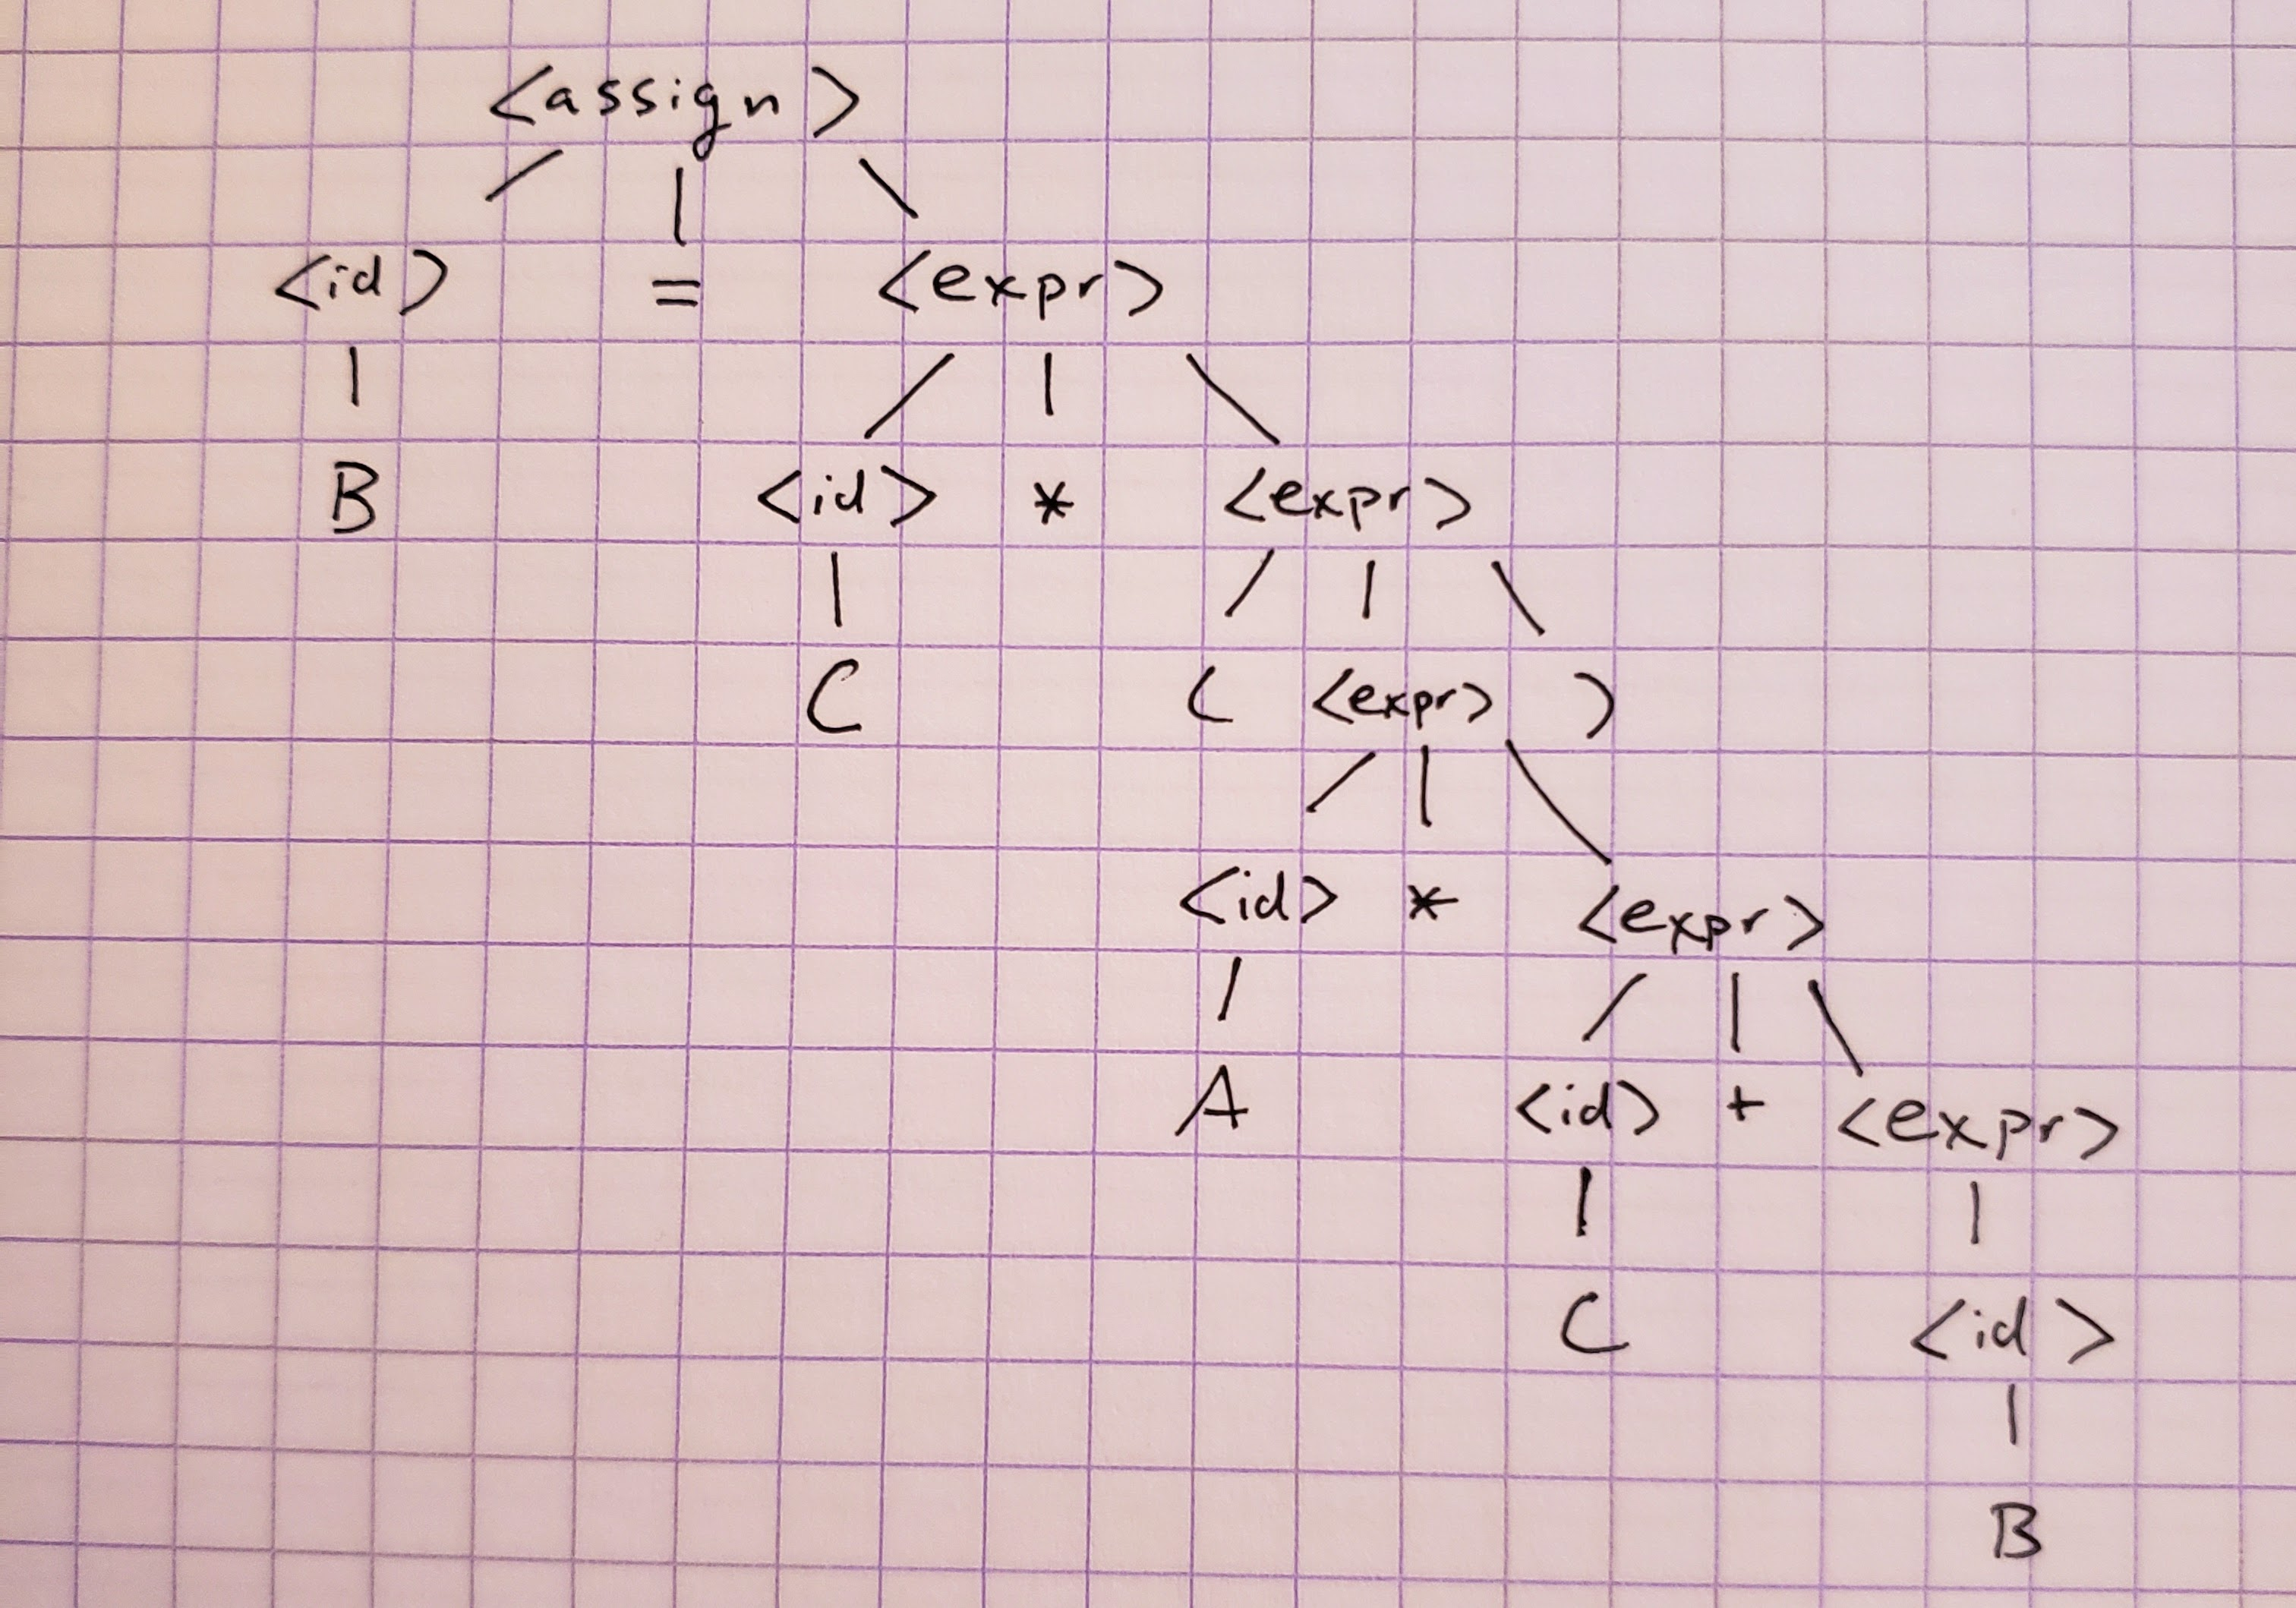
\includegraphics[width=\textwidth]{hw02tree2.jpg}
\caption{Parse tree for question 2}
\label{fig:tree2}
\end{figure}

\newpage
\hwnumbersec{3}{7(a)}

\begin{minipage}{0.8\textwidth}
\centering
\begin{grammar}
	<assign> $\implies$\\
	<id> = <expr> \\
	$\implies$ A = <term> * <factor> \\
	$\implies$ A = <term> * <id>\\
	$\implies$ A = <term> * C\\
	$\implies$ A = <factor> * C\\
	$\implies$ A = (<expr>) * C\\
	$\implies$ A = (<expr> + <term>) * C\\
	$\implies$ A = (<expr> + <factor>) * C\\
	$\implies$ A = (<expr> + <id>) * C\\
	$\implies$ A = (<expr> + B) * C\\
	$\implies$ A = (<term> + B) * C\\
	$\implies$ A = (<factor> + B) * C\\
	$\implies$ A = (A + B) * C
\end{grammar}
\end{minipage}

Parse tree:
\begin{figure}[h]
\centering
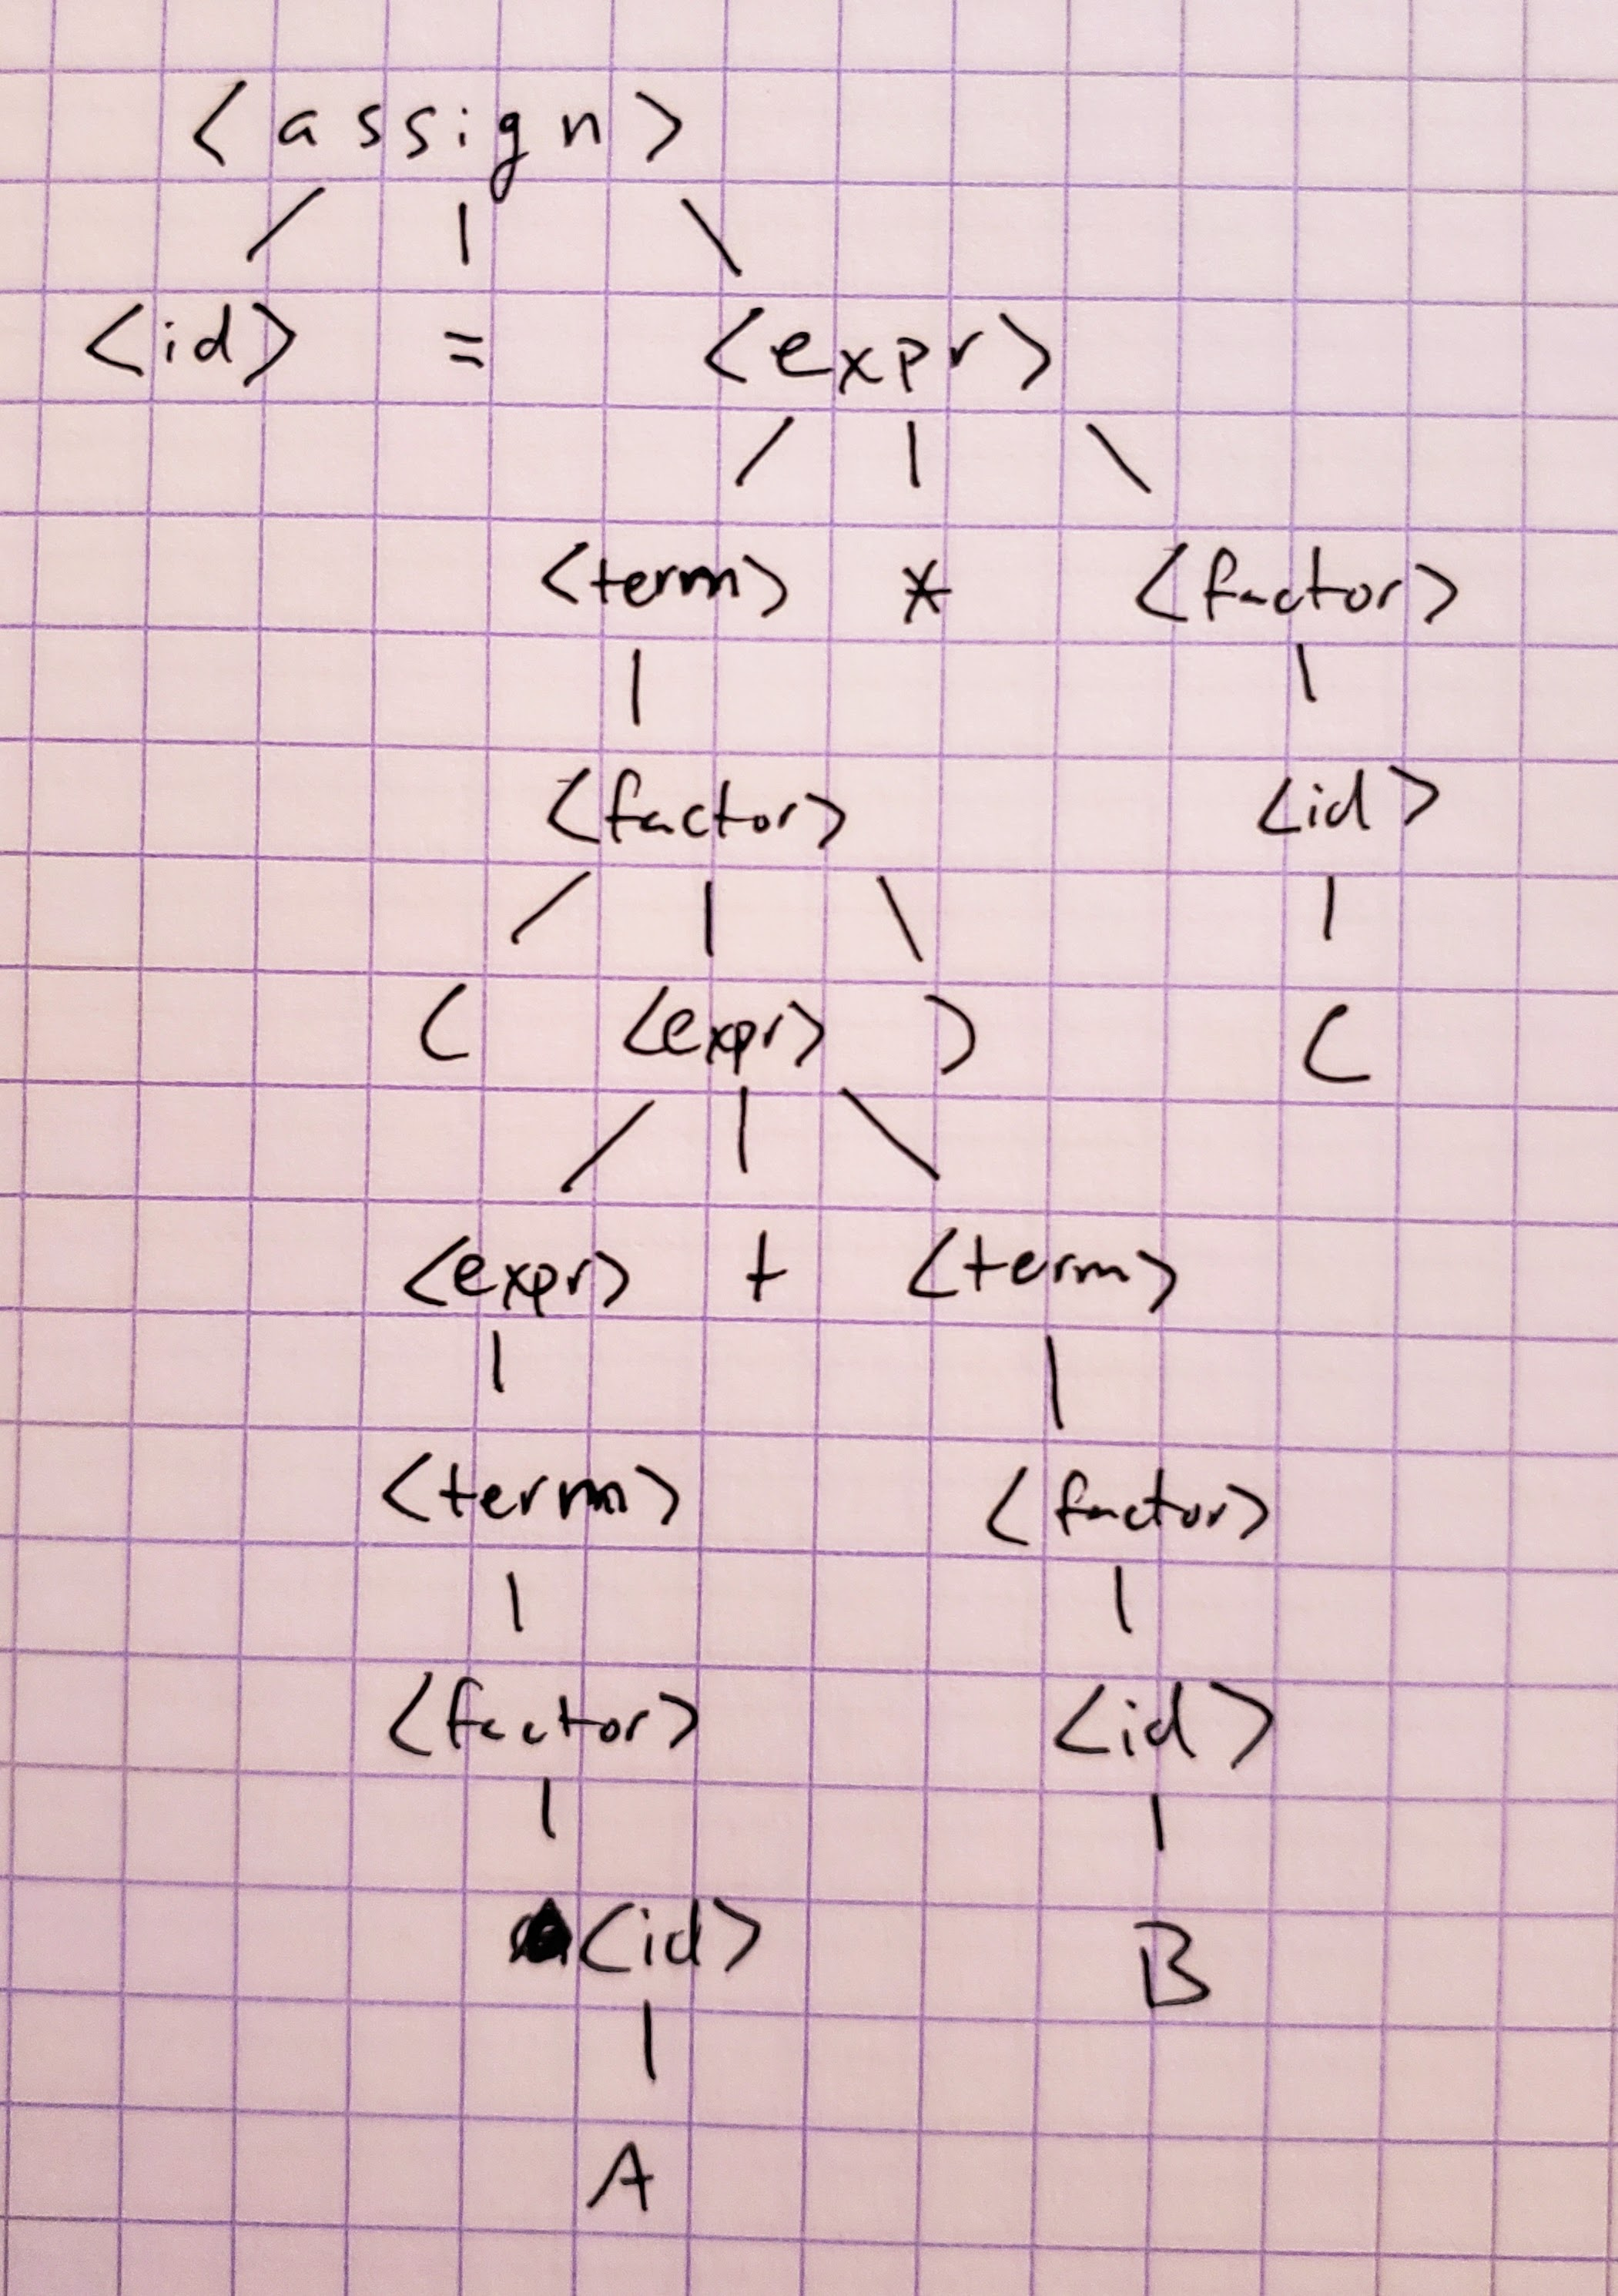
\includegraphics[scale=0.07]{hw02tree3.jpg}
\caption{Parse tree for question 3}
\label{fig:tree3}
\end{figure}


\newpage
\hwnumbersec{4}{11}

The strings \texttt{baab} and \texttt{bbaab} are valid, but \texttt{bbbab} and
\texttt{bbaaaaa} are not. 

\hwnumbersec{5}{15}

We have the following EBNF grammar:
\medskip

\begin{minipage}{0.8\textwidth}
\centering
\begin{grammar}
	<program> \To \texttt{begin} <stmt_list> \texttt{end}\\
	<stmt_list> \To <stmt> \{; <stmt_list>\}\\
	<stmt> \To <var = <expression>\\
	<var> \To A | B | C\\
	<expression> \To <var> \{(+ | -) <var> \}
\end{grammar}
\end{minipage}

\hwnumbersec{6}{17}

We have the following BNF grammar:
\medskip

\begin{minipage}{0.8\textwidth}
	\centering
	S \To SbA $\vert$ A \\
	A \To aA $\vert$ abA
\end{minipage}

\hwnumber{7}{23(a and b)}

\textbf{(a)}

\begin{align*}
	&2 * (b - 1) - 1 > 0 \\
	&2 * (b - 1) > 1 \\
	&(b - 1) > \frac{1}{2}\\
	&b > \frac{3}{2}
\end{align*}

So the weakest precondition is $b > \frac{3}{2}$
\medskip

\textbf{(b)}

\begin{align*}
	&\frac{c + 10}{3} > 6\\
	&c + 10 > 18 \\
	&c > 8
\end{align*}

So the weakest precondition is $c > 8$.


\end{document}
